
\paragraph{Esempio MQS}
Si consideri un sistema di spire e nuclei magnetici, in questo caso due gioghi magnetici sui quali
vengono posti due avvolgimenti, rappresentati con una spira singola in figura.
\begin{figure}[H]
\centering
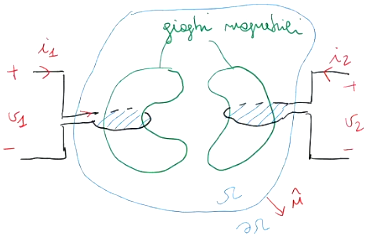
\includegraphics[width = 0.5\linewidth]{gioghi_magnetici}
\end{figure}
Si considera la superficie $\Omega$ con frontiera $\partial \Omega$ e si applica il bilancio energetico
$$
-\iint_{\partial\Omega} \vec{S}\cdot\hat{n}dS = v_1i_1 + v_2i_2 = \frac{dw_m}{dt}
$$
Applicando Faraday-Neumann alle spire orientate come le correnti $i_1$ e $i_2$
$$
-v_1 = -\frac{d\Phi_1}{dt}\qquad -v_2 = -\frac{d\Phi_2}{dt}
$$
sostituendo nella precedente, in forma differenziale, si ottiene
$$
\left(v_1i_1 + v_2i_2\right)dt = dw_m \Rightarrow i_1d\Phi_1 + i_2d\Phi_2 = dw_m = \frac{\partial w_m}{\partial \Phi_1}d\Phi_1 + \frac{\partial w_m}{\partial \Phi_2}d\Phi_2
$$
$$
w_m\left(\Phi_1,\Phi_2\right)\qquad i_1 = \frac{dw_m}{d\Phi_1}\qquad i_2 = \frac{dw_m}{d\Phi_2}
$$
Essendo $\Phi_1$ e $\Phi_2$ grandezze di stato per la variabile $w_m$ si può immaginare di risolvere
l'integrale come in un piano termodinamico
$$
w_m(\Phi_1,\Phi_2) = \int_0^{\Phi_1} i_1d\Phi_1' + \int_0^{\Phi_2} i_2 d\Phi_2'
$$
In figura sono mostrati i possibili percorsi per raggiungere lo stato $(\Phi_1,\Phi_2)$ partendo da una
condizione di riposo $(0,0)$
\begin{figure}[H]
\centering
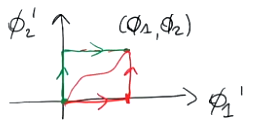
\includegraphics[width = 0.4\linewidth]{percorsi_flussi}
\end{figure}
\newpage
Si ricapitolano le espressioni dell'energia immagazzinata in funzione della carica e dei flussi di corrente
$$
w_e(Q) = \int_0^Q v(Q')dQ'\qquad w_m\left(\Phi_1,\Phi_2\right) = \int_0^{\Phi_1}i_1(\Phi_1',\Phi_2')d\Phi_1' + 
\int_0^{\Phi_2}i_1(\Phi_1',\Phi_2')d\Phi_2'
$$
\subsection{Coenergia}
Si vuole ottenere l'espressione dell'energia magnetica in funzione delle correnti e non dei flussi, allo
stesso modo l'energia elettrica in funzione della tensione e non della carica.

Si considera il modello EQS, si considera la cosiddetta \href{https://en.wikipedia.org/wiki/Coenergy}{\textit{COENERGIA}}
$$
\delta(vQ) = v\delta Q + Q\delta v = dw_e + dw_e'\qquad dw_e' = Q\delta v\quad \text{coenergia elettrica}
$$
$$
dw_e' = \delta(vQ) - dw_e \Rightarrow w_e'(v) = v\cdot Q - \int_0^Q v(Q')dQ'
$$
la coenergia è funzione di $v$ se si riesce ad esprimere la carica $Q$ in funzione della tensione.

Caso MQS, si ripetono gli stessi step, si ricava la coenergia magnetica $w_m'$
$$
\delta(i_1\Phi_1 + i_2\Phi_2) = i_1d\Phi_1 + i_2d\Phi_2 + \Phi_1di_1 + \Phi_2di_2 = dw_m + dw_m'
$$
$$
dw_m' = \Phi_1di_1 + \Phi_2di_2 \Rightarrow w_m'(i_1,i_2) = \int_0^{i_1} \Phi_1(i_1',i_2')di_1' + \int_0^{i_2} \Phi_2(i_1',i_2')di_2'
$$
\subparagraph{Esempio MQS lineare}
Si considera il circuito magnetico a due spire precedentemente presentato, tra le due spire saranno
presenti i coefficienti di mutua induzione ed autoinduzione.
$$\begin{aligned}
\Phi_1 &= L_1i_1 + M_{12}i_2\\
\Phi_2 &= M_{21}i_1 + L_2i_2
\end{aligned}
$$
Si costruisce $w_m'$ nel piano $(i_1',i_2')$ eseguendo due integrali monodimensionali su linee rette come
rappresentato in figura.
\begin{figure}[H]
\centering
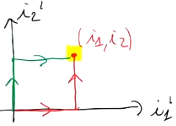
\includegraphics[width=0.3\linewidth]{integrale_flussi_stati}
\end{figure}
Percorso rosso
$$
w_m'(i_1,i_2) = \int_0^{i_1}\Phi_1(i_1',i_2'=0) di_1' + \int_0^{i_2} \Phi_2(i_1,i_2')di_2' = \frac{1}{2}L_1i_1^2 + M_{21}i_1i_2 + \frac{1}{2}L_2i_2^2
$$

Percorso verde
$$
w_m'(i_1,i_2) = \int_0^{i_2}\Phi_2(i_1'=0,i_2)di_2' + \int_0^{i_1}\Phi_1(i_1',i_2)di_1' = \frac{1}{2}L_2i_2^2 + \frac{1}{2}L_1i_1^2 + M_{12}i_1i_2
$$
$M_{12}$ deve necessariamente essere pari ad $M_{21}$ affinché i due stati coincidano.
\newpage

\subsection{Sistemi conservativi con un grado di libertà meccanico}
Sistemi rigidi dotati di moto monodimensionale.
Si immagina di poter compiere lavoro meccanico al sistema nella forma generale
$$
dL = fd\xi \qquad f\text{ forza}\qquad \xi \text{ spostamento}
$$
nel bilancio energetico
$$
p_\text{in} = v\cdot i = dw + fd\xi
$$
Il termine $dw$ è la variazione di energia interna, $fd\xi$ è il lavoro meccanico che il sistema compie. Manca 
l'energia dissipata perché si è fatta l'ipotesi di sistema conservativo.

Caso EQS
$$
vdQ = dw_e + fd\xi \Rightarrow dw_e = vdQ - fd\xi
$$
$$
w_e(Q,\xi) \Rightarrow v= \frac{\partial w_e}{\partial Q}\qquad f=-\frac{\partial w_e}{\partial \xi}
$$
Le ultime due relazioni costituiscono il \href{https://it.wikipedia.org/wiki/Teorema_dei_lavori_virtuali}{Principio dei Lavori Virtuali} dal quale si deriva che dato un sistema rigido ad un grado di libertà, sia dato uno
spostamento infinitesimo $d\xi$ arbitrario attorno al punto di equilibrio, si può dunque valutare la forza
necessaria a compiere il generico spostamento valutando la derivata dell'energia rispetto allo spostamento
$$
f = -\frac{\partial w_e}{\partial \xi}
$$

Ad esempio, per costruire $w_e$ si può fare un integrale nello spazio di stato $(Q,\xi)$ lungo i percorsi del ``taxi''
$$
w_e(Q,\xi) = -\cancel{\int_0^\xi f(Q'=0,\xi')d\xi'} + \int_0^Qv(Q',\xi)dQ'
$$
il primo termine è zero dato che se il condensatore è scarico, non c'è nessuna forza che si oppone allo spostamento
dunque il lavoro è nullo, il secondo termine è invece calcolato a spostamento costante.
\newpage
\paragraph{Esempio EQS} Condensatore parzialmente riempito di dielettrico, classico microfono capacitivo, trasduttore 
elettromeccanico che trasforma le onde meccaniche (sonore) che colpiscono l'armatura in segnale elettrico.
Si vede in figura lo schema del condensatore parzialmente riempito dal dielettrico con una delle due armature mobili.
\begin{figure}[H]
\centering
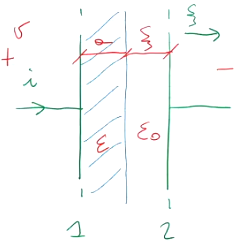
\includegraphics[width = 0.3\linewidth]{condensatore_parziale_dielettrico}
\end{figure}
Si ricava la forza presente tra le armature ricordando che la tensione tra le armature è pari a
$$
v(Q',\xi)=\frac{Q}{C(\xi)}
$$
l'energia dunque
$$
w_e(Q) = \int_0^Qv(Q',\xi)dQ' = \int_0^Q\frac{Q'}{C(\xi)}dQ' = \frac{1}{2}\frac{Q^2}{C(\xi)}
$$
la capacità può essere vista come la capacità di due condensatori in serie, uno con dielettrico ed uno mobile
senza dielettrico, per il principio di metallizzazione delle superfici equipotenziali
$$
C(\xi) = \left(\frac{1}{\frac{\varepsilon S}{a}} +  \frac{1}{\frac{\varepsilon_0 S}{\xi}}\right)^{-1} =
\frac{a\varepsilon_0S + \xi\varepsilon S}{\varepsilon S^2 \varepsilon_0}^{-1} = 
\frac{\varepsilon S^{\cancel{2}} \varepsilon_0}{a\varepsilon_0\cancel{S} + \xi\varepsilon \cancel{S}} =
\frac{\varepsilon\varepsilon_0S}{a\varepsilon_0 + \xi\varepsilon}
$$

con la relazione di Maxwell
$$
f = -\frac{\partial w_e}{\partial \xi} = -\frac{1}{2}Q^2\frac{\partial}{\partial\xi}\left(\frac{1}{C(\xi)}\right)=
\frac{1}{2}\frac{Q^2}{C^2}\frac{\partial C}{\partial\xi} = \frac{1}{2}v^2\frac{\partial C}{\partial\xi} = -\frac{1}{2}v^2\frac{\varepsilon^2\varepsilon_0S}{\left(a\varepsilon_0+\xi\varepsilon\right)^2}
$$
dal segno si vede che la forza si oppone allo spostamento positivo, dunque è una forza di attrazione tra le
armature.
La pressione invece
$$
\frac{f}{S} = p = -\frac{1}{2}\varepsilon_0 E^2
$$
è formalmente uguale alla densità di energia elettrostatica.
\newpage
\paragraph{Esempio MQS} Si suppone di avere due avvolgimenti (per semplicità)
$$
i_1d\Phi_1 + i_2d\Phi_2 = dw_m + fd\xi
$$
dove $d\xi$ è uno spostamento generico nel sistema, dell'avvolgimento o di qualsiasi altra parte.
$$
dw_m = i_1d\Phi_1 + i_2d\Phi_2 - fd\xi\Rightarrow w_m\left(\Phi_1,\Phi_2,\xi\right)
$$
$$
i_1 = \frac{\partial w_m}{\partial \Phi_1}\qquad i_2 = \frac{\partial w_m}{\partial \Phi_2}\qquad f = -\frac{\partial w_m}{\partial \xi}
$$
Si consideri una linea bifilare schematizzata da due conduttori cilindrici indefiniti di raggio $a$
posti alla distanza $\xi$
\begin{figure}[H]
\centering
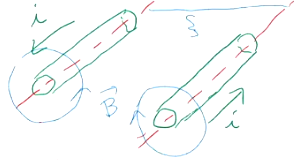
\includegraphics[width = 0.3\linewidth]{linea_bifilare_MQS}
\end{figure}
l'induttanza per unità di lunghezza è
$$
\frac{L}{l} = \frac{\mu_0}{\pi} \ln\left(\frac{\xi}{a}\right)
$$
nell'ipotesi in cui il raggio $a$ sia molto minore della distanza $\xi$.

Il flusso concatenato 
$$
\Phi = Lli = \frac{\mu_0}{\pi}i \ln\left(\frac{\xi}{a}\right)l
$$
L'energia sarà
$$
w_m(\Phi,\xi) = \int_0^\Phi i(\Phi')d\Phi' = \frac{1}{2}\frac{\Phi^2}{L(\xi)}
$$
La forza tra i due conduttori
$$
f = -\frac{\partial w_m}{\partial \xi} = \frac{\Phi^2}{2}\frac{1}{L^2(\xi)}\frac{\partial L}{\partial \xi} =
\frac{i^2}{2}\frac{\mu_0}{\pi}\frac{\cancel{a}}{\xi}\frac{1}{\cancel{a}} l =
\frac{i^2}{2}\frac{\mu_0}{\pi}\frac{l}{\xi}
$$
In questo caso la forza è repulsiva perché concorde allo spostamento.
La stessa espressione si può ricavare con la legge di Lorentz.
\newpage
\subsection{Forza di un elettromagnete}
Si consideri un giogo a C avvolto da $N$ spire percorse da una corrente $i$, posto in vicinanza
di una barra di ferro dolce che può traslare lungo un asse, posta a distanza $\xi$ dal giogo.
\begin{figure}[H]
\centering
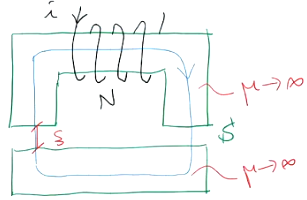
\includegraphics[width = 0.4\linewidth]{elettromagnete_MQS}
\end{figure}
Sia $S$ la sezione del traferro, si applica la legge di Hopkinson
$$
Ni = \mathcal{R}\Phi_1 \Rightarrow \Phi = N\Phi_1 = \frac{N^2}{\mathcal{R}(\xi)}i
$$
con la riluttanza nel traferro pari a
$$
\mathcal{R}(\xi) = \frac{2\xi}{\mu_0 S}
$$
l'energia magnetica
$$
w_m(\Phi,\xi) = \frac{\Phi^2}{2L(\xi)} = L(\xi)\cdot i
$$
applicando l'equazione di Maxwell
$$
f = -\frac{\partial w_m}{\partial \xi} = \frac{1}{2}i^2 \frac{\partial L}{\partial \xi} =
\frac{1}{2}i^2\frac{\partial}{\partial \xi} \left[\frac{N^2\mu_0 S}{2\xi}\right] = 
-\frac{1}{4}i^2\frac{N^2\mu_0 S}{\xi^2}
$$
La forza aumenta quadraticamente al ridursi dello spessore del traferro.

Si ricava ancora la legge di Hopkinson al traferro
$$
Ni = 2H_t\xi = 2\frac{B_t}{\mu_0}\xi
$$
Dunque il campo al traferro è dato da
$$
B_t = \frac{\Phi}{S} = \frac{\mu_0Ni}{2\xi} 
$$
quindi l'espressione della forza si può riscrivere in funzione del campo al traferro $B_t$
$$
f = -\frac{1}{2}\frac{\left(\frac{iN}{2\xi}\mu_0\right)^2}{\mu_0} \cdot 2S = -\frac{1}{2}\frac{B_t^2}{\mu_0}\cdot2S
= p_m2S
$$
con $p_m = -\frac{1}{2}\frac{B_t^2}{\mu_0}$ la pressione magnetica
\newpage
\paragraph{Elettromagnete con magnete permanente}
Si ha un magnete permanente collegato a due espansioni polari di sezione $S$, si vuole calcolare la forza di 
attrazione su un giogo mobile.
\begin{figure}[H]
\centering
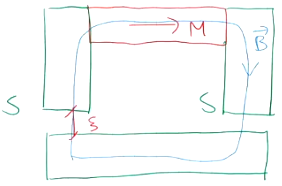
\includegraphics[width = 0.4\linewidth]{magnete_permanente_giogo}
\end{figure}
Le equazioni del sistema sono:
$$\begin{aligned}
&B_mS_m = \Phi_m = \Phi_t = B_tS_t\\
&2H_t\xi + l_mH_m = 0
\end{aligned}
$$
\begin{figure}[H]
\centering
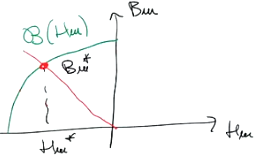
\includegraphics[width=0.3\linewidth]{curva_magnete_permanente}
\end{figure}
La curva rossa è la seconda equazione mentre la verde è la caratteristica del magnete
$$
B_m = \mathcal{B}(H_m)
$$
Il punto di lavoro $(B_m^*,H_m^*)$ è l'intersezione tra le due ed è funzione dello spostamento $\xi$

La forza è dunque
$$
f = -\frac{1}{2\mu_0}B_t^2 = -\frac{{B_m^*}^2(\xi){S_m}^2}{2\mu_0 {S_t}^2}
$$
equazione non lineare che va risolta numericamente al variare della posizione del giogo mobile
dato che, come si ricava dalle equazioni precedenti
$$
B_t = B_m^*(\xi)\frac{S_m}{S_t}
$$

\newpage
\subsection{Macchina elettrica rotante}
Il lavoro compiuto da una coppia di forze uguali e opposte, su un corpo rigido, produce un momento $\tau$
ed una rotazione $d\theta$
$$
fd\xi \rightarrow \tau d\theta
$$
Si rappresenta lo schema di una macchina elettrica rotante, sintetizzata come un cilindro cavo
di materiale ferromagnetico, chiamato \textit{statore}, sul quale sono avvolte delle spire come mostrato in figura
\begin{figure}[H]
\centering
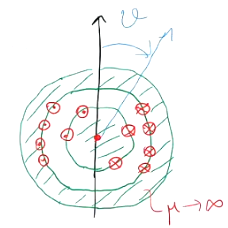
\includegraphics[width = 0.35\linewidth]{macchina_elettrica}
\end{figure}
All'interno dello statore è posto un altro cilindro di materiale ferromagnetico dolce sul quale è posto
un altro avvolgimento.

Si suppone che nella condizione iniziale l'avvolgimento del rotore sia ruotato di un certo angolo
$\theta$ rispetto allo statore; il cilindro del rotore ha un raggio $b$ mentre il raggio interno dello 
statore è invece $a$.

Se
$$
fd\xi \rightarrow f = \frac{\partial w_m'}{\partial\xi}
$$
allora
$$
\tau d\theta \rightarrow \tau= \frac{\partial w_m'}{\partial \theta}
$$
ricordando che 
$$
dw_m' = \Phi_1di_1 + \Phi_2di_2 + fd\xi
$$
si può ricavare analogamente la formula per lo spostamento angolare
$$
dw_m' = \Phi_1di_1 + \Phi_2di_2 + fd\theta
$$
integrando
$$
w_m'(i_1,i_2,\theta) = \frac{1}{2}L_1i_1^2 +  \frac{1}{2}L_2i_2^2 + M(\theta)i_1i_2
$$
i coefficienti $L_1$ ed $L_2$ non dipendono da $\theta$ essendo di auto-induzione
$$
\tau = \frac{\partial w_m'}{\partial \theta} = i_1i_2\frac{\partial M}{\partial \theta}
$$
supponendo che 
$$
M(\theta) = M^*\cos\theta
$$
ossia che l'accoppiamento sia massimo quando gli avvolgimenti sono allineati, mentre $M^*$ si potrebbe
calcolare misurando il campo $B$ al traferro pressoché radiale.

$\tau$ dipende anche da $i_1(t)$ e $i_2(t)$ quindi con la stessa macchina è possibile realizzare
sia un motore che un generatore, a seconda del segno della coppia.

\subparagraph{Macchina sincrona} Utilizzata per realizzare motori sincroni o alternatori, si
suppone la corrente $i_1$ di statore sinusoidale mentre la corrente $i_2$ nel rotore costante.
Supponendo che la velocità angolare $\omega$ del rotore sia costante, l'angolo $\theta$ sarà
$$
\omega t - \alpha
$$
dunque la coppia istantanea 
$$
\tau = i_1(t)i_2(t) \frac{\partial M}{\partial \theta} = -I_1\cos\left(\omega t\right) I_2 M^* \sin\left(\Omega t - \alpha\right)
$$
con la \href{https://it.wikipedia.org/wiki/Formule_di_Werner}{formula di Werner}
$$
\cos\left(x\right)\sin\left(y\right) = \frac{1}{2}\left( \sin\left(x+y\right) + \sin\left(x-y\right) \right)
$$
la $\tau$ diventa
$$
\tau = -\frac{I_1I_2}{2}M^*\left[\sin\left(\left(\omega+\Omega\right)t - \alpha\right) +
\sin\left(\left(\Omega-\omega\right)t-\alpha\right)\right]
$$
il valor medio
$$
\frac{1}{T}\int_0^T \tau dt' = <\tau>_T \neq 0 \text{ se e solo se } \Omega = \omega
$$
ossia la pulsazione della corrente di alimentazione dello statore deve essere identica alla velocità angolare
del rotore. In quest'ipotesi
$$
<\tau>_T = \frac{I_1I_2}{2}M^*\sin\alpha \
\begin{aligned}
&\diagup > 0 \text{ se } \alpha \ \in\ (0,\pi) \text{ motore} \\
&\diagdown < 0 \text{ se } \alpha \ \in\ (\pi,2\pi) \text{ generatore}
\end{aligned}
$$
Si rappresenta in figura il momento magnetico dello statore, che ruota attorno all'asse al variare
della corrente per il teorema di \href{https://it.wikipedia.org/wiki/Campo_magnetico_alternato_e_rotante}{Galileo Ferraris}. Anche il momento magnetico del rotore ruota, nonostante la corrente sia costante a causa della
rotazione meccanica del rotore.
\begin{figure}[H]
\centering
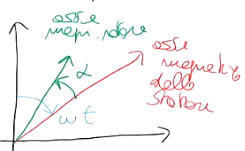
\includegraphics[width = 0.4\linewidth]{assi_magnetici}
\end{figure}
L'angolo $\alpha$ è dunque l'angolo di ritardo tra i due assi magnetici.
